% =====================================================================
% THIS FILE IS THE SOURCE. Rebuild with:
%     bash tools/compile.sh Unit_06_Causal_and_Data_Provenance
%
% Unit 6 merges the old Causal Thinking and Where the Data Comes From
% decks. They both taught selection bias separately, once as a collider
% and once as survivorship, so the merged unit teaches the mechanism once
% and then shows both faces of it.
% =====================================================================
% THIS FILE IS THE SOURCE. Edit it, then rebuild the PDF with:
%     bash tools/compile.sh Unit_05_Causal_Thinking
% (run from the Course_Rewrite folder; it compiles twice and reports
%  page count, overfull boxes, and em dashes)
%
% Do not edit the PDF directly. Figures are the fig_*.pdf files in this
% folder, regenerated by tools/make_module*_slide_figs.py.
%
% Originally converted from the 15-module draft by a one-shot script now
% parked in tools/one_shot_generators/. Re-running those would discard
% anything you change here, so they are kept out of tools/ on purpose.
% =====================================================================
\documentclass[aspectratio=169]{beamer}
\usetheme{default}
\usefonttheme{professionalfonts}
\usepackage{amsmath, amssymb, amsfonts}
\usepackage{graphicx}
\usepackage{booktabs}
% more air between table rows, they run together otherwise
\renewcommand{\arraystretch}{1.2}
\usepackage{array}
\newcolumntype{L}[1]{>{\raggedright\arraybackslash}p{#1}}
\usepackage{bm}
\usepackage{hyperref}

\mode<presentation> {
    \usetheme{Frankfurt}
    \usecolortheme{default}
}

\newcommand{\xbar}{\bar{x}}
\newcommand{\yhat}{\hat{y}}

\newenvironment{principle}[1]{\begin{block}{\textbf{Principle:} #1}}{\end{block}}
\newenvironment{trap}[1]{\begin{alertblock}{\textbf{Trap:} #1}}{\end{alertblock}}
\newenvironment{practice}[1]{\begin{exampleblock}{\textbf{In practice:} #1}}{\end{exampleblock}}
\newenvironment{interview}[1]{\begin{exampleblock}{\textbf{You may be asked:} #1}}{\end{exampleblock}}
\newenvironment{yourturn}[1]{%
  \setbeamercolor{block title}{fg=white,bg=orange!80!black}%
  \setbeamercolor{block body}{bg=orange!12}%
  \begin{block}{\textbf{Your turn:} #1}}{\end{block}}
\newenvironment{livedemo}[1]{%
  \setbeamercolor{block title}{fg=white,bg=teal!80!black}%
  \setbeamercolor{block body}{bg=teal!12}%
  \begin{block}{\textbf{Live demo:} #1}}{\end{block}}
\newenvironment{llmcheck}[1]{%
  \setbeamercolor{block title}{fg=white,bg=violet!75!black}%
  \setbeamercolor{block body}{bg=violet!10}%
  \begin{block}{\textbf{LLM check:} #1}}{\end{block}}

\title{Where the Data Came From}
\subtitle{Unit 6: Causal Claims, Selection, and What You Are Allowed to Conclude}
\author{Stat 220 \textbar{} Statistics for Data Science}
\date{}

\begin{document}

\begin{frame}
  \titlepage
\end{frame}

\section{Why}

\begin{frame}{Where this fits}
\begin{itemize}
  \item Units 3 through 5 built models, judged them honestly, and put error bars on what they
        predict. All of that assumed the rows in front of you were the rows you should have.
  \item This unit asks the two questions that come before any of it. Where did these rows come
        from, and does the pattern in them mean what it looks like?
  \item Those turn out to be one question. A confounder and a biased sample are both cases of the
        data being assembled in a way that plants a pattern you did not put there.
\end{itemize}
\begin{principle}{the order that matters}
No amount of modeling fixes a dataset that answers a different question than the one you asked.
The check happens first, or it does not happen.
\end{principle}
\end{frame}

\begin{frame}{What this unit gives you}
\begin{columns}[T]
\begin{column}{0.5\textwidth}
\textbf{Things to know}
\begin{itemize}\small
  \item what a causal effect is, in terms of what would have happened otherwise
  \item why randomization works, and exactly what it buys
  \item the three roles a third variable can play, and what to do about each
  \item that colliders and survivorship bias are one mechanism
  \item population, sampling frame, and the designs worth knowing
  \item how data goes missing, and what that does to your answer
\end{itemize}
\end{column}
\begin{column}{0.5\textwidth}
\textbf{Mistakes to stop making}
\begin{itemize}\small
  \item controlling for everything you have
  \item reading a slope from observational data as an effect
  \item treating sample size as evidence of representativeness
  \item studying only the survivors, winners, or responders
  \item dropping missing rows without asking why they are missing
  \item accepting a proxy as the thing you meant to measure
\end{itemize}
\end{column}
\end{columns}
\end{frame}


\section{Effects}

\begin{frame}{An effect is a comparison with something that never happened}
\begin{itemize}
  \item For one customer, the effect of the discount is: what they spend \emph{with} it, minus what
        they would have spent \emph{without} it.
  \item You can only ever observe one of those two. The other is a counterfactual, and it is
        missing by definition.
  \item So causal inference is a \textbf{missing data problem}: everything hinges on how you fill
        in the world that did not happen.
\end{itemize}
\begin{principle}{the question behind every causal claim}
``Compared to what?'' If someone cannot tell you what their comparison group is, they do not have
a causal estimate.
\end{principle}
\end{frame}


\begin{frame}{Why randomization is the gold standard}
\begin{itemize}
  \item Randomly assigning treatment makes the two groups comparable \emph{in expectation} on
        everything: age, motivation, prior spending, and every variable you never thought to
        measure.
  \item That last clause is the important one. Adjustment can only handle confounders you
        measured. Randomization handles the ones you did not.
  \item What it does \emph{not} fix: small samples, dropout after assignment, non-compliance,
        contaminated control groups, or measuring the wrong outcome.
\end{itemize}
\begin{practice}{say this precisely}
``Randomization does not make the groups identical. It makes any difference between them the kind
of difference we can quantify with a standard error.''
\end{practice}
\end{frame}


\section{Third variables}

\begin{frame}{The three roles a third variable can play}
\begin{center}
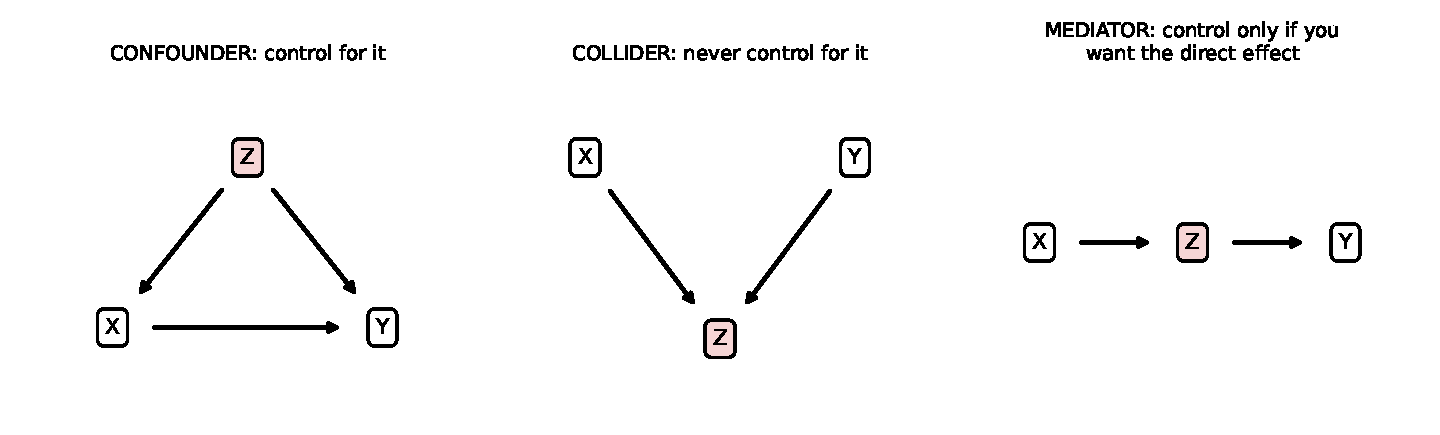
\includegraphics[width=0.98\textwidth]{fig_m12_dags.pdf}
\end{center}
\vspace{-0.2em}
\small
The arrows are what you believe about the world. Which variables to control for is decided by these
diagrams, \emph{not} by which ones improve the fit.
\end{frame}


\begin{frame}{Confounders: the classic problem}
\begin{itemize}
  \item A \textbf{confounder} causes both the treatment and the outcome, producing an association
        with no causal path behind it.
  \item Ice cream sales and drownings both rise with temperature. Neither causes the other.
  \item In business: customers who \emph{choose} the premium plan were already more engaged, so
        premium looks like it causes retention.
\end{itemize}
\begin{principle}{control for confounders, and say which ones you could not measure}
The honest sentence is: ``adjusting for tenure, plan size, and industry, the difference is X, but
I cannot rule out that more motivated teams chose the feature.''
\end{principle}
\end{frame}


\begin{frame}{Confounding in real data}
\begin{center}
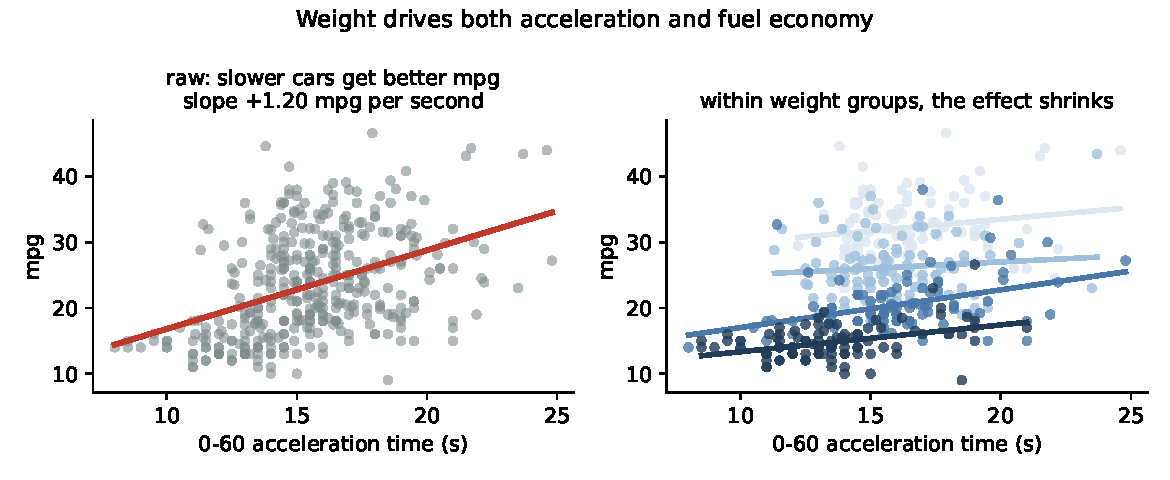
\includegraphics[width=0.9\textwidth]{fig_m12_confounder.pdf}
\end{center}
\vspace{-0.4em}
\small
392 cars. Slower-accelerating cars average \textbf{1.20 mpg better per extra second} to 60. Once
you adjust for weight, which drives both, the association collapses to \textbf{0.26}. Nearly 80\%
of the raw relationship was weight, relabeled.
\end{frame}


\begin{frame}{Colliders}
\begin{itemize}
  \item A \textbf{collider} is caused by both variables. Conditioning on it creates an association
        where none existed, exactly as the dice demonstrated.
  \item Selecting your sample on a collider is the same mistake: analyzing only customers who
        \emph{contacted support}, only patients who were \emph{admitted}, only startups that
        \emph{got funded}.
  \item This is why ``add every variable you have to the regression'' is bad advice. Some of those
        variables are colliders, and adding them injects bias rather than removing it.
\end{itemize}
\begin{trap}{the kitchen-sink regression}
More controls is not safer. Each control is a claim about the causal diagram, and the wrong one
makes your estimate worse in a direction you cannot sign.
\end{trap}
\end{frame}


\begin{frame}{Mediators}
\begin{itemize}
  \item A \textbf{mediator} sits on the causal path: training raises skill, skill raises sales.
  \item If you regress sales on training \emph{controlling for skill}, you have removed the very
        channel through which training works, and the effect vanishes.
  \item Controlling for a mediator answers a different, narrower question: is there a direct effect
        \emph{other than} through skill?
\end{itemize}
\begin{practice}{a question that trips people up}
``Should you control for everything?'' The right answer is no, and the reason is exactly this:
confounders yes, colliders never, mediators only if you deliberately want the direct effect.
\end{practice}
\end{frame}


\begin{frame}{The rules, in one table}
\begin{center}\small
\begin{tabular}{p{0.20\textwidth} p{0.30\textwidth} p{0.38\textwidth}}
\toprule
\textbf{Role} & \textbf{Structure} & \textbf{What to do} \\
\midrule
Confounder & causes both $X$ and $Y$ & \textbf{Control for it.} Omitting it biases the
estimate. \\
Collider & is caused by both $X$ and $Y$ & \textbf{Never control for it}, and never select the
sample on it. \\
Mediator & $X$ causes it, it causes $Y$ & \textbf{Leave it out} for the total effect. \\
\bottomrule
\end{tabular}
\end{center}
\vspace{0.4em}
\begin{principle}{the order of operations}
Decide the role from what you believe about the world, \emph{then} write the model. You cannot
read the role off a correlation matrix, and the fit will not tell you either.
\end{principle}
\end{frame}


\begin{frame}{Your turn \#1}
\begin{yourturn}{classify the variable}
You want the effect of a \textbf{new onboarding flow} on 90-day retention. For each variable, say
whether you should control for it, and why:
\begin{enumerate}
  \item Company size at signup.
  \item Number of features used in week one.
  \item Whether the customer contacted support at any point.
\end{enumerate}
\end{yourturn}
\end{frame}


\begin{frame}{Your turn \#1: answer}
\begin{itemize}
  \item \textbf{Company size:} a confounder. It affects both which flow they got (if assignment was
        not random) and retention. \textbf{Control for it.}
  \item \textbf{Features used in week one:} a mediator. That is how onboarding works.
        \textbf{Do not control} unless you specifically want the effect that runs through some
        other channel.
  \item \textbf{Contacted support:} a collider. It is caused by both the onboarding experience and
        by the customer's underlying trouble. \textbf{Never control for it}, and do not restrict
        the sample to those who contacted support.
\end{itemize}
\begin{principle}{draw the arrows before you write the formula}
Two minutes with a diagram prevents a month of arguing about a coefficient.
\end{principle}
\end{frame}


\section{Selection}

\begin{frame}{Colliders and survivorship bias are the same thing}
You have now met the collider: conditioning on a common consequence of two variables makes them
look related when they are not. That mechanism has other names depending on who got filtered out.
\begin{center}\small
\renewcommand{\arraystretch}{1.05}%
\begin{tabular}{L{0.24\textwidth} L{0.32\textwidth} L{0.34\textwidth}}
\toprule
\textbf{Name} & \textbf{What got filtered} & \textbf{The pattern it plants} \\
\midrule
Collider bias & cases that scored high on a shared consequence & two unrelated causes look
  negatively related \\
Survivorship bias & anything that did not last & the traits of survivors look like the causes of
  survival \\
Nonresponse bias & people who chose not to answer & the answers you got look like the answers
  everyone would give \\
\bottomrule
\end{tabular}
\end{center}
\begin{principle}{one question covers all three}
Ask who is missing from this table, and what it took to get in. That single question catches every
row above.
\end{principle}
\end{frame}


\begin{frame}{Selection can create a relationship}
\begin{center}
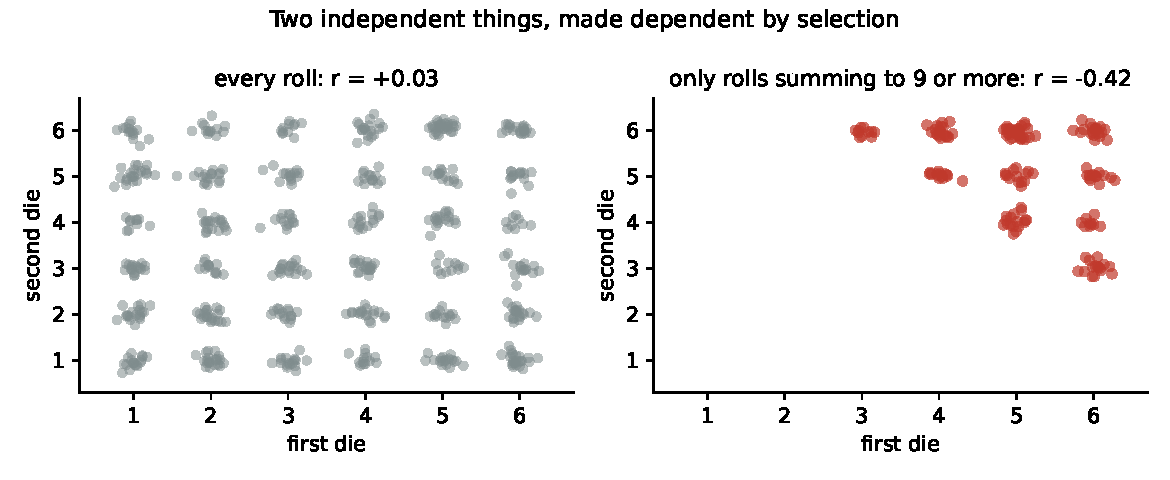
\includegraphics[width=0.92\textwidth]{fig_m12_collider.pdf}
\end{center}
\vspace{-0.4em}
\small
Independent to begin with. Among high-sum rolls, a low first die \emph{requires} a high second
die, so the two become strongly negatively related. Nothing about the dice changed. We changed who
was in the dataset.
\end{frame}


\begin{frame}{Where this shows up in real data}
\begin{itemize}
  \item Restaurants you hear about are either great food or great location, because bad on both
        close. So in your data, food quality and location look negatively related.
  \item Admitted students are either strong on tests or strong on essays. Within the admitted
        class, the two look like they trade off.
  \item Hospitalized patients have some serious condition, so among them, unrelated diseases appear
        connected.
\end{itemize}
\begin{principle}{the sample is part of the analysis}
Before you interpret any relationship, ask who got into the dataset, and what it took to get in.
\end{principle}
\end{frame}


\begin{frame}{Survivorship bias}
\begin{center}
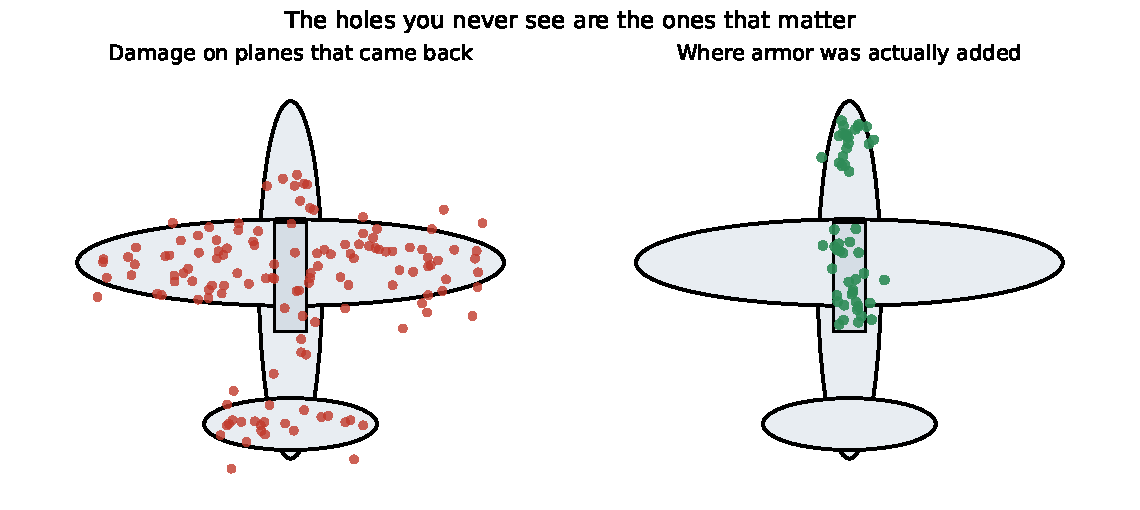
\includegraphics[width=0.84\textwidth]{fig_m14_survivorship.pdf}
\end{center}
\vspace{-0.4em}
\small
In World War II, analysts studied bullet holes in returning bombers and proposed armoring the
wings, where the holes were. Abraham Wald pointed out the obvious once you see it: those planes
came back. Armor belongs where the returning planes have \emph{no} holes, because planes hit there
did not return.
\end{frame}


\begin{frame}{Nonresponse}
\begin{columns}[c]
\begin{column}{0.58\textwidth}
\centering
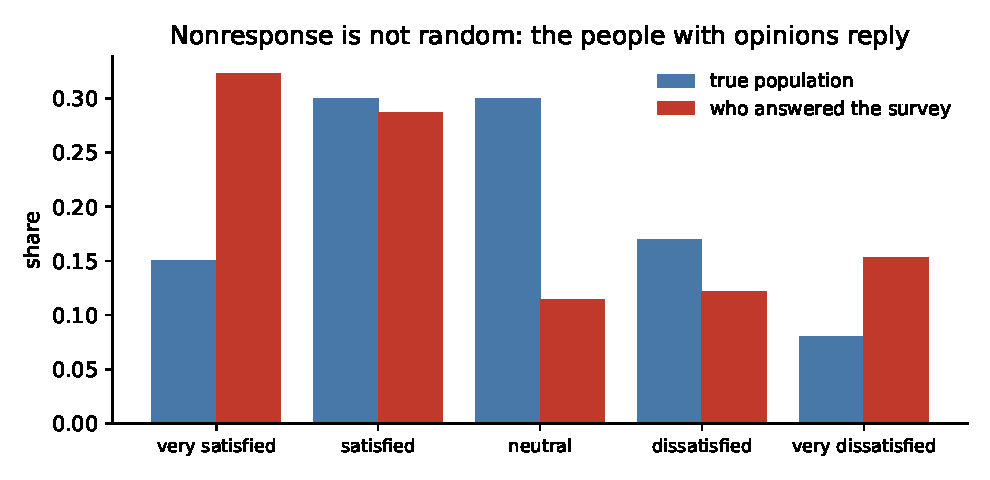
\includegraphics[width=\textwidth]{fig_m14_nonresponse.pdf}
\end{column}
\begin{column}{0.42\textwidth}
\small
People with strong feelings answer surveys. The indifferent middle does not.
\begin{itemize}
  \item Your satisfaction data becomes bimodal even when the population is not.
  \item Response rates for phone polls have fallen from over 30\% to under 10\%, and the tilt is
        what makes modern polling hard.
\end{itemize}
\end{column}
\end{columns}
\onslide<2->{\centering\small
Weighting can correct for \emph{measured} differences. It cannot correct for people who differ in
ways you did not record.}
\end{frame}


\begin{frame}{Two famous failures}
\begin{itemize}
  \item \textbf{1936:} the \emph{Literary Digest} mailed 10 million ballots and got 2.4 million
        back, predicting a Landon landslide. Roosevelt won 46 states. The frame came from car and
        telephone registries in the Depression, and only the enthusiastic mailed back.
  \item At the same time George Gallup polled about 50{,}000 people, chosen to match the
        population, and got it right.
  \item \textbf{The lesson repeats:} 2.4 million biased responses lost to 50{,}000 designed ones.
\end{itemize}
\begin{principle}{design beats volume}
Sampling error shrinks with $n$. Sampling bias does not shrink at all.
\end{principle}
\end{frame}


\begin{frame}{The big-data paradox}
\begin{columns}[c]
\begin{column}{0.58\textwidth}
\centering
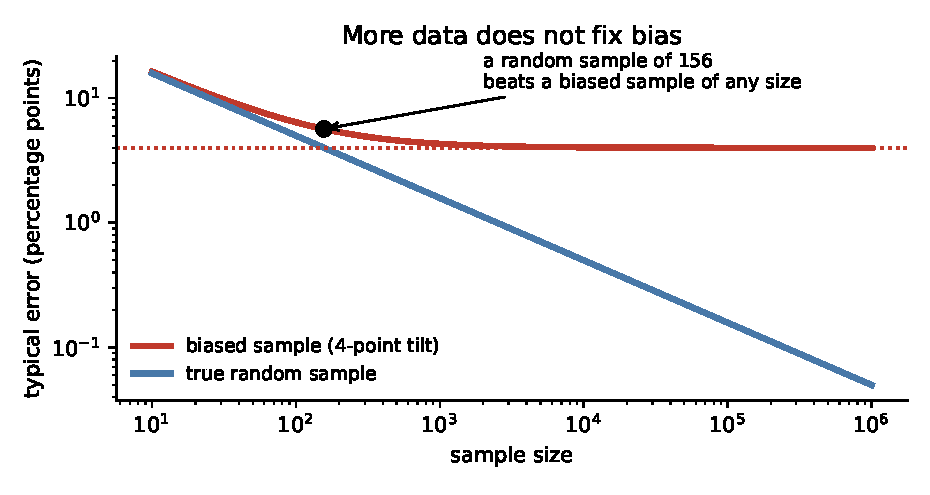
\includegraphics[width=\textwidth]{fig_m14_bias_vs_n.pdf}
\end{column}
\begin{column}{0.42\textwidth}
\small
A sample with a 4-point systematic tilt never gets more accurate than 4 points, however many rows
you add.
\begin{itemize}
  \item A \emph{random} sample of about \textbf{156} matches it.
  \item Worse: the huge sample reports a tiny standard error, so it is confidently wrong.
\end{itemize}
\end{column}
\end{columns}
\onslide<2->{\centering\small
This is exactly how 40 million app users can mislead you about your market.}
\end{frame}


\section{Provenance}

\begin{frame}{Population, frame, sample}
\begin{itemize}
  \item \textbf{Population:} everyone you want to describe. All customers, all flights, all voters.
  \item \textbf{Sampling frame:} the list you can actually draw from. Your CRM, the phone book,
        people with app notifications enabled.
  \item \textbf{Sample:} who ended up in the data.
\end{itemize}
Bias enters at both arrows: frame does not match population (\textbf{undercoverage}), and sample
does not match frame (\textbf{nonresponse}).
\begin{principle}{name your frame out loud}
``Our customers'' usually means ``customers with an email on file who opened the message.'' Saying
the real frame is often enough to spot the problem.
\end{principle}
\end{frame}


\begin{frame}{Four sampling designs}
\begin{itemize}
  \item \textbf{Simple random sample:} everyone equally likely. The benchmark.
  \item \textbf{Stratified:} split into groups (region, plan tier), sample within each. More
        precision for the same cost, and guarantees small groups appear.
  \item \textbf{Cluster:} sample whole groups (stores, classrooms) and measure everyone inside.
        Cheaper, but the effective sample size is closer to the number of clusters.
  \item \textbf{Systematic:} take every $k$th record. Fine unless the list has a hidden periodicity.
\end{itemize}
\begin{trap}{cluster samples analyzed as if they were random}
Surveying 20 stores with 50 customers each is not 1{,}000 independent observations. Treating it as
such is the standard-error error from Unit 9, at scale.
\end{trap}
\end{frame}


\begin{frame}{Your turn \#2}
\begin{yourturn}{find the frame problem}
A streaming service estimates ``average weekly viewing hours per subscriber'' from telemetry sent
by its smart-TV app.
\vspace{0.3em}

With a neighbor: name three groups of subscribers this misses or distorts, and say which direction
the estimate is biased.
\end{yourturn}
\end{frame}


\begin{frame}{Your turn \#2: answer}
\begin{itemize}
  \item Subscribers who watch on phones, laptops, or game consoles are missing entirely, and their
        habits differ.
  \item Households sharing one account look like one heavy viewer, while a subscriber who never
        opens the app sends no telemetry at all and may vanish from the denominator.
  \item Anyone with telemetry disabled, or an older TV, is excluded, and both correlate with age
        and income.
\end{itemize}
\begin{principle}{ask what the instrument can see}
Telemetry measures device activity, not people watching. The gap between those two is where the
bias lives.
\end{principle}
\end{frame}




\begin{frame}{Missing values in real data}
\begin{center}
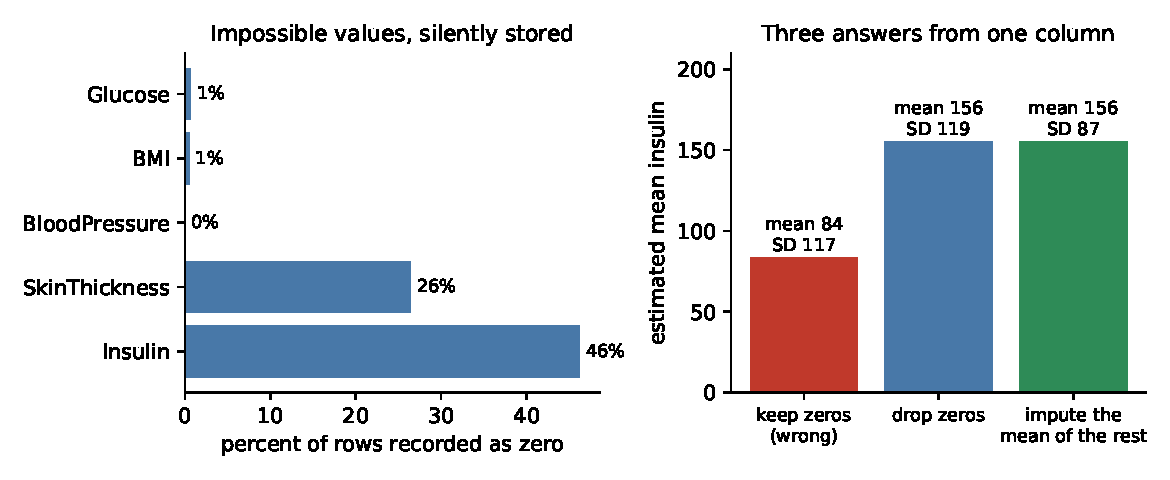
\includegraphics[width=0.92\textwidth]{fig_m14_missing.pdf}
\end{center}
\vspace{-0.4em}
\small
733 patients. Insulin is recorded as zero for \textbf{46\%} of them, which is biologically
impossible: those are missing values recorded as zero. Keeping them halves the estimated mean.
Mean imputation gets the mean right and shrinks the SD from 119 to 87, manufacturing precision that
does not exist.
\end{frame}


\begin{frame}{Three ways data goes missing}
\begin{itemize}
  \item \textbf{Missing completely at random:} the machine failed randomly. Dropping rows costs
        precision but is unbiased. Rare in practice.
  \item \textbf{Missing at random (given what you measured):} older patients skip a test more often,
        and you recorded age. Dropping is biased. Modeling with age is not.
  \item \textbf{Missing not at random:} the value itself drives the absence. High earners refuse to
        report income, and the sickest patients miss follow-up. Nothing in the data fixes this. You need
        external information or an explicit assumption.
\end{itemize}
\begin{trap}{silent listwise deletion}
Most software drops incomplete rows without telling you. If the dropped rows differ systematically,
your entire analysis quietly changed populations.
\end{trap}
\end{frame}


\begin{frame}{What to actually do}
\begin{enumerate}
  \item \textbf{Count and map the missingness} first, per column, and check whether missing rows
        differ from complete ones on the outcome.
  \item \textbf{Look for disguised codes}: 0, $-1$, 999, ``N/A'', or an empty string.
  \item \textbf{Add a missingness indicator} when absence itself might be informative. Often it is
        the most predictive feature you have.
  \item \textbf{Prefer multiple imputation} to single mean imputation, so the extra uncertainty
        shows up in the interval instead of vanishing.
  \item \textbf{Say what you did}, and show the result both ways.
\end{enumerate}
\end{frame}


\begin{frame}{Weighting}
When your sample's composition is wrong but you \emph{know} the true composition, you can reweight.
\begin{center}\footnotesize
\renewcommand{\arraystretch}{1.05}%
\begin{tabular}{lccc}
\toprule
\textbf{Age group} & \textbf{\% of population} & \textbf{\% of respondents} & \textbf{weight} \\
\midrule
18--34 & 30\% & 12\% & 2.50 \\
35--54 & 35\% & 33\% & 1.06 \\
55+    & 35\% & 55\% & 0.64 \\
\bottomrule
\end{tabular}
\end{center}
\vspace{0.4em}
\begin{itemize}
  \item Each young respondent now counts for 2.5 people, so the estimate reflects the population
        mix rather than who answered.
  \item It only fixes imbalance on variables you \emph{measured}, and heavy weights inflate the
        variance.
\end{itemize}
\begin{trap}{weighting as a blank check}
``We weighted the survey'' does not mean the bias is gone. It means the bias on the weighting
variables is gone.
\end{trap}
\end{frame}


\begin{frame}{You measure a proxy, not the concept}
\begin{itemize}
  \item ``Engagement'' becomes clicks. ``Teacher quality'' becomes test scores. ``Customer
        happiness'' becomes a survey score from the 6\% who responded.
  \item Every proxy has a gap between it and the real concept, and decisions get made in that gap.
  \item \textbf{Goodhart's law:} once a proxy becomes a target, people optimize the proxy, and the
        gap widens on purpose.
\end{itemize}
\begin{practice}{a strong thing to raise unprompted}
``Before I model this, what exactly does this column measure, who recorded it, and when? Half the
projects I have seen went wrong at that step.''
\end{practice}
\end{frame}


\begin{frame}{Measurement problems that look like findings}
\begin{itemize}
  \item \textbf{Instrument drift:} a logging change in March makes April look like a behavior shift.
  \item \textbf{Question wording:} ``Do you support banning X?'' and ``Do you oppose allowing X?''
        give different numbers from identical people.
  \item \textbf{Social desirability:} people over-report voting, exercise, and reading. They
        under-report drinking and screen time.
  \item \textbf{Definition changes:} a churn spike caused by moving the churn cutoff from 90 to 60
        days.
\end{itemize}
\begin{trap}{check the instrument before the world}
Before explaining a sudden jump with a story about the world, check whether the instrument changed
on that date. It usually did.
\end{trap}
\end{frame}


\begin{frame}{Your turn \#3}
\begin{yourturn}{whose data is it?}
A hiring team builds a model to predict "good employees" using performance ratings from the past
ten years of hires.
\vspace{0.3em}

With a neighbor: identify one selection problem, one measurement problem, and one missing-data
problem in that setup.
\end{yourturn}
\end{frame}


\begin{frame}{Your turn \#3: answer}
\begin{itemize}
  \item \textbf{Selection:} you only observe performance for people who were \emph{hired}. Rejected
        candidates who would have excelled are invisible, so the model learns the old process's
        preferences.
  \item \textbf{Measurement:} ``performance rating'' is a manager's judgment, carrying whatever
        biases and grade inflation that manager had. It is a proxy, not the concept.
  \item \textbf{Missing:} people who left early have no rating, and they left for reasons related
        to the outcome. That is missing not at random.
\end{itemize}
\begin{principle}{the model inherits the process that made the data}
A model trained on past decisions predicts the past decisions, including their mistakes. That is
not a bug you can regularize away.
\end{principle}
\end{frame}


\section{Quasi-experiments}

\begin{frame}{When you cannot randomize}
Often you cannot randomize: it is unethical, illegal, too slow, or the change already happened.
Four workhorse designs, each buying credibility with an assumption:
\begin{itemize}
  \item \textbf{Matching / adjustment:} compare treated units to similar untreated ones.
        \emph{Assumes} you measured every confounder.
  \item \textbf{Difference in differences:} compare changes over time against a control group.
        \emph{Assumes} the two groups would have moved in parallel.
  \item \textbf{Regression discontinuity:} compare units just above and just below a cutoff.
        \emph{Assumes} units cannot precisely manipulate their position.
  \item \textbf{Instrumental variables:} use a nudge that affects treatment but nothing else.
        \emph{Assumes} the instrument has no other path to the outcome.
\end{itemize}
\end{frame}


\begin{frame}{Difference in differences, drawn}
\begin{columns}[c]
\begin{column}{0.58\textwidth}
\centering
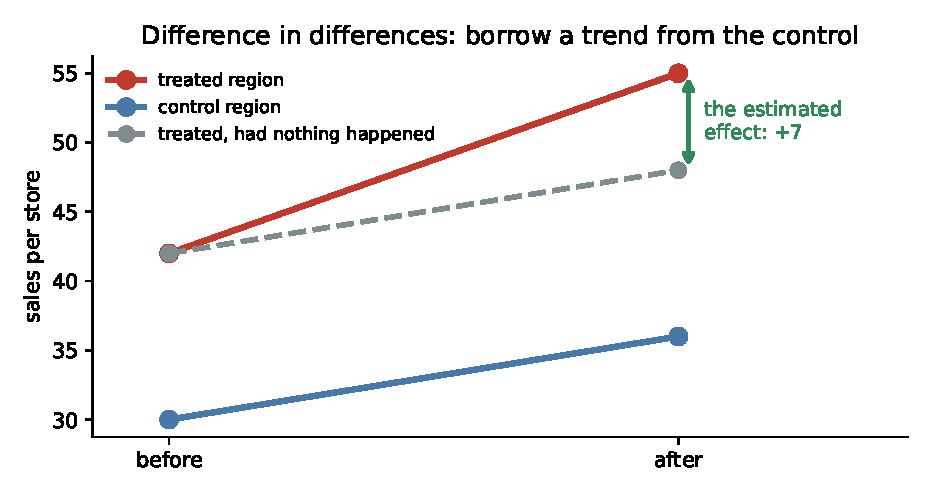
\includegraphics[width=\textwidth]{fig_m12_did.pdf}
\end{column}
\begin{column}{0.42\textwidth}
\small
The treated region rose by 13. But the control region rose by 6 without any treatment, so the
economy was moving anyway.
\begin{itemize}
  \item Estimated effect: $13 - 6 = \textbf{7}$.
  \item Everything rests on the dashed line, the claim that the treated region would have followed
        the control's trend.
\end{itemize}
\end{column}
\end{columns}
\onslide<2->{\centering\small
So the first thing to check is whether the two lines were parallel \emph{before} the change.}
\end{frame}


\begin{frame}{Difference in differences, with the actual arithmetic}
A chain raises pay in its \textbf{Ohio} stores in July and leaves \textbf{Indiana} alone.
\begin{center}\small
\renewcommand{\arraystretch}{1.05}%
\begin{tabular}{lccc}
\toprule
 & \textbf{before} & \textbf{after} & \textbf{change} \\
\midrule
Ohio (treated)    & 42.0 & 55.0 & $+13.0$ \\
Indiana (control) & 30.0 & 36.0 & $+6.0$ \\
\midrule
\textbf{difference in differences} & & & $\mathbf{+7.0}$ \\
\bottomrule
\end{tabular}
\end{center}
\vspace{0.4em}
\begin{itemize}
  \item Ohio rose 13, but 6 of that would have happened anyway. The estimated effect is
        \textbf{7}.
  \item It all rests on the claim that Ohio \emph{would have} risen by 6 too, which is untestable
        after treatment.
\end{itemize}
\begin{principle}{how to check what you cannot test}
Plot both series for several periods \emph{before} the change. If they moved together then, the
assumption is credible.
\end{principle}
\end{frame}


\begin{frame}{Reverse causation, and how to rule it out}
\begin{itemize}
  \item Hospitals with more staff have higher mortality. Do nurses kill people, or do sicker
        patients get more nurses?
  \item Ad spend and sales move together, partly because budgets are \emph{set} as a percentage of
        expected sales.
  \item Police numbers and crime, tutoring and grades, maintenance and failures: in each case the
        outcome plausibly causes the treatment.
\end{itemize}
\begin{principle}{the fix is timing, not statistics}
Establish that the cause moved \emph{first}, and for a reason unrelated to the outcome. That is
what a rollout date, a policy change, or a budget freeze gives you, and no regression can
substitute for it.
\end{principle}
\end{frame}


\begin{frame}{Natural experiments}
\begin{itemize}
  \item \textbf{John Snow, 1854:} two water companies served interleaved houses on the same London
        streets, one drawing from sewage-contaminated water. The houses were otherwise alike, so
        the cholera difference was as good as randomized.
  \item \textbf{Minimum wage, 1994:} Card and Krueger compared fast-food employment in New Jersey
        after a wage increase against neighboring Pennsylvania, a difference in differences that
        reversed the textbook prediction.
  \item \textbf{Scholarship cutoffs:} students just above and just below a score threshold are
        nearly identical, so the cutoff acts like a coin flip.
\end{itemize}
\begin{principle}{look for the accident}
The best observational studies find a moment where something outside the actors' control assigned
the treatment for them.
\end{principle}
\end{frame}


\begin{frame}{Your turn \#4}
\begin{yourturn}{design the study}
Your company rolled out a new sales-training program. Reps who completed it sold 18\% more last
quarter than reps who did not. Leadership wants to make it mandatory.
\vspace{0.3em}

With a neighbor: name two reasons that 18\% may not be the effect of training, and design a study
you could actually run next quarter.
\end{yourturn}
\end{frame}


\begin{frame}{Your turn \#4: answer}
\begin{itemize}
  \item \textbf{Selection:} reps who volunteered were more motivated, and would have improved
        anyway. \textbf{Regression to the mean:} if struggling reps were assigned, expect a bounce
        with no cause.
  \item \textbf{Timing:} the quarter may have been better for everyone, which a simple before-after
        comparison would credit to training.
  \item \textbf{The study:} randomize the next cohort. If that is impossible, use a staged rollout
        by region and compare with difference in differences, checking that the regions were
        parallel beforehand.
\end{itemize}
\begin{principle}{staged rollouts are free experiments}
If you must launch to everyone eventually, launch in a random order. It costs nothing and converts
a guess into an estimate.
\end{principle}
\end{frame}


\section{LLM check}

\begin{frame}{LLM check: mistake or not? (1 of 2)}
\begin{llmcheck}{we asked an LLM about a feature launch}
\textbf{We told it:} ``Customers who use our new dashboard renew at 91\%, others at 68\%. What is
the effect of the dashboard on renewal?''\\[4pt]
\textbf{It answered:} ``The dashboard increases renewal by 23 percentage points. To be thorough I
would control for every variable available in your database to remove any confounding.''
\end{llmcheck}
\vspace{0.2em}
\centering\small Mistake, or no mistake?
\onslide<2->{%
\begin{trap}{verdict: mistake, twice}
First, the 23 points is a comparison between customers who \emph{chose} the dashboard and those who
did not, so it is mostly selection. Second, ``control for everything'' is wrong: some of those
variables are colliders and mediators, and controlling for them adds bias.
\end{trap}}
\end{frame}


\begin{frame}{LLM check: mistake or not? (2 of 2)}
\begin{llmcheck}{we asked an LLM about sample size}
\textbf{We told it:} ``Our survey of app users got 40,000 responses out of 2 million invitations.
Is that enough to represent our user base?''\\[4pt]
\textbf{It answered:} ``Yes, 40,000 is an excellent sample size. The margin of error is under 0.5\%,
so you can be very confident these results represent your users.''
\end{llmcheck}
\vspace{0.2em}
\centering\small Mistake, or no mistake?
\onslide<2->{%
\begin{trap}{verdict: mistake}
A 2\% response rate is the headline, not the 40{,}000. The margin of error describes sampling
error only, and says nothing about the 98\% who did not answer. The tiny stated error makes the
result more dangerous, not more trustworthy.
\end{trap}}
\end{frame}


\section{Consolidate}

\begin{frame}{How to answer ``does X cause Y?''}
\begin{enumerate}
  \item \textbf{State the intervention precisely.} Who gets what, instead of what?
  \item \textbf{Name the comparison group.} If there is none, stop.
  \item \textbf{Draw the diagram}: candidate confounders, colliders, mediators.
  \item \textbf{Ask how treatment was assigned.} Randomized, chosen, or assigned by a rule?
  \item \textbf{Choose the design} that fits the assignment mechanism.
  \item \textbf{Check the design's assumption} explicitly (parallel pre-trends, balance, no
        manipulation at the cutoff).
  \item \textbf{Report the effect with its uncertainty and its caveats}, including the confounder
        you could not measure.
\end{enumerate}
\end{frame}


\begin{frame}{An audit to run first}
\small
\begin{enumerate}
  \item \textbf{Name the population} the decision concerns, and the frame the rows actually came from.
  \item \textbf{Ask who is missing because of the outcome} you are studying.
  \item \textbf{Count the missing values per column}, and look for them in disguise: 0, $-1$, 999, empty strings.
  \item \textbf{Compare rows with missing values to complete rows} on the outcome. If they differ, dropping them changes the population.
  \item \textbf{Ask what each column really measures}, who recorded it, and when.
  \item \textbf{Check for breaks over time} in the instrument, the definition, or the pipeline.
  \item \textbf{Write down what you could not fix}, and put it in the report.
\end{enumerate}
\end{frame}


\begin{frame}{The traps, all in one place}
\begin{trap}{the ones that bite most often}
\begin{itemize}
  \item Reading a slope from observational data as an effect.
  \item Controlling for everything available, which is how you condition on a collider.
  \item Controlling for a mediator and then reporting the effect as if it vanished.
  \item Treating a large sample as a representative one.
  \item Studying only survivors, winners, or people who responded.
  \item Dropping rows with missing values without asking why they are missing.
  \item Imputing the mean and then quoting the narrower interval that results.
  \item Accepting a proxy as the concept you actually meant.
\end{itemize}
\end{trap}
\end{frame}


\begin{frame}{What you should be able to do with software}
\small
Nobody is asking you to memorize syntax. You are expected to know \emph{which} procedure the
question calls for, what to hand it, and what the output means. With an AI assistant open, you
should be able to produce any of these and defend the result.
\begin{center}\footnotesize
\renewcommand{\arraystretch}{1.05}%
\begin{tabular}{p{0.44\textwidth} p{0.46\textwidth}}
\toprule
\textbf{You should be able to} & \textbf{What you would reach for} \\
\midrule
Adjusted comparison & \texttt{smf.ols(\"y \textasciitilde\ treat + covariates\", data)} \\
Estimates within strata & \texttt{pd.qcut} then \texttt{groupby} \\
Difference in differences & four group means, then the difference of the differences \\
Check parallel pre-trends & plot both series for several periods before treatment \\
Randomized assignment for a rollout & \texttt{rng.integers(0, 2, n)} on the unit of assignment \\
Simulate a confounder or a collider & generate the data yourself and compare estimates \\
Logistic version for a binary outcome & \texttt{smf.logit} \\
\bottomrule
\end{tabular}
\end{center}
\vspace{0.2em}
\centering\small
If you cannot say what the output means, the fact that you produced it is worth nothing.
\end{frame}


\begin{frame}{Where we go next}
\begin{itemize}
  \item That closes Part I. You can build a model, judge it honestly, say how wrong a prediction
        might be, and now ask whether the data ever supported the claim.
  \item Part II goes back and earns the machinery. \textbf{Unit 7} starts with probability, which
        is what the standard errors, the $p$-values, and the distributions have been resting on
        the whole time.
\end{itemize}
\begin{principle}{the through-line}
Part I was about what you can conclude. Part II is about why those tools are entitled to conclude
anything at all.
\end{principle}
\end{frame}


\end{document}
